\documentclass[../main.tex]{subfiles}
\begin{document}
\subsection{Колмогоровская сложность моделей}

Одним из фундаментальных способов определить сложность произвольного математического объекта является колмогоровская сложность. Ниже представлено формальное определение колмогоровской сложности и основные ее свойства.


\begin{definition}
Пусть задано вычислимое частично определенное отображение из множества бинарных слов в себя:
\[
T: \{0,1\}^{*}  \to  \{0,1\}^{*}.
\]
Колмогоровской сложностью бинарной строки $x$ назовем минимальную длину описания относительно $T$:
\[
K_T(x) = \min_{f \in \{0,1\}^*}\{|f|: T(f) = x\},
\]
\end{definition}
Заметим, что колмогоровская сложность зависит от отображения $T$. В~\cite{kolmogorov} доказано, что колмогоровсксая сложность $K_T(x)$ при двух отображениях $T_1, T_2$ отличается лишь на некоторую константу, не зависящих от строки $x$. Поэтому для дальнейшего изложения зафиксируем некоторое отображение $T$ и положим $K(x) = K_T(x)$.


\begin{figure}
\centering
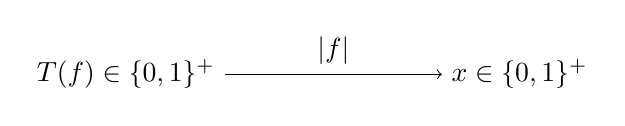
\begin{tikzpicture}[node distance=cm, auto]
  %\tikzstyle{every state}=[fill=red,draw=none,text=white]
  \node (x)  at (1,3)                  {$T(f) \in \{0,1\}^{+}$};
  \node (f)  at (6,3)                  {$x \in \{0,1\}^{+}$};
\path[->]  (x) edge  node   {$\argmin |f|$} (f);

\end{tikzpicture}

\caption{}
\end{figure}


Обобщим понятие колмогоровской сложности на случай двух бинарных строк.

\begin{definition}
Пусть задано вычислимое и частично определенное отображение из декартового произведения двух множеств бинарных слов в себя:
\[
T: \{0,1\}^{*} \times  \{0,1\}^{*} \to  \{0,1\}^{*}.
\]

Условной колмогоровской сложностью бинарной строки $y$ при условии $x$ назовем минимальную длину описания относительно $T$:
\[
K_T(y|x) = \min_{f \in \{0,1\}^*}\{|f|: T(f, y) = x\},
\]
\end{definition}
Аналогично простой колмогоровской сложности, зафиксируем некоторое отображение $T$ и положим $K_T(y|x) = K(y|x)$.

Рассмотрим некоторые свойства условной колмогоровской сложности.


\textbf{Оценка условной Колмогоровской сложности}~\cite{kolmogorov}
\[
	K(x,y) \leq K(x) + K(y|x) + O(\log K(x,y)).
\]


\textbf{Количество информации в паре x,y симметрично с точностью до константы}:
\[
I(x:y) = I(y:x) + O(\text{log}K(x,y)),
\]
где величина $I(x:y) = K(y) - K(y|x)$  задает количество информации в $x$ об объекте $y$. 

Отметим, что схожими свойствами обладает взаимная информация и энтропия, определения которых даны ниже.

\begin{definition}
Пусть задана дискретная случайная величина $x$ с вероятностным распределением $p$, принимающая значения $x_1, \dots, x_n$,
Энтропией распределения случайной величины $x$ назовем:
\[
	H(x) = -\sum_{i=1}^n p(x = x_i) \log~p(x = x_i).
\]
\end{definition}
\textbf{Оценка условной энтропии}
\[
	H(x,y) = H(x) + K(y|x).
\]
\begin{definition}
Взаимной информацией $I$ двух случайных величин $x,y$ назовем следующее выражение:
\[
	I(x,y) = H(x) - H(x|y), \quad H(x) = - \sum_{i} p_x(x_i) \log p_x(x_i)ю
\]
\end{definition}
\textbf{Взаимная информация симметрична}:
\[
I(x,y) = I(y,x).
\]

Таким образом, свойства энтропии и колмогровской сложности, а также количества информации $I(x:y)$ и взаимной информации, во многом совпадают. Докажем теорему о связи колмогоровской сложности и энтропии распределения, подытоживающую связь этих двух математических объектов.

\begin{theorem}~\cite{kolmogorov}
Пусть задана некоторая строка $x$ длины $n$ с частотами  $p = (p_0, 1 - p_0)$ появлений нулей и единиц в строке.
Тогда
\[
K(x) \leq H(x) + O(\log m).
\]
Неравенство обращается в равенство для большинства строк $x$ длины $n$.
\end{theorem}
\begin{proof}
Всего слов, которые можно получить с использованием заданных частот:
\[
    C = \frac{m!}{(p_0 m)! ((1-p_0)m)! }.
\]
Т.к. количество таких слов конечно, то их можно пронумеровать и построить отображение, выдающее строку $x$ по ее порядковому номеру.
Таким образом, условная колмогоровская сложность ограничена сверху:
\[
K(x|C, p_0) \leq \log C + O(1).
\]
Воспользуемся формулой Стирлинга:
\[
    n! = \sqrt{(2\pi + o(1))n}\bigl(\frac{n}{e}^n\bigr).
\]
И получим оценку:
\[
    C \leq 2^{nH(x) + O(\log n)}, \quad K(x|C, p_0) \leq  nH(x) + O(\log n).
\]

Для того, чтобы избавиться от условия в $K(x|C, p_0)$  потребуется $O(\log n)$ бит для описания чисел $p_0n, n$.

TODO: Поскольку слов с более короткими описаниями меньше, чем $C$, то для большинства слов будет достигаться предложенная оценка.
\end{proof}

Частным случаем колмогоровской сложности является префиксная колмогоровская  сложность. Эта сложность задается машиной Тьюринга специального вида, имеющей две ленты: однонаправленную ленту для чтения и двунаправленную рабочую ленту. Будем полагать что машина Тьюринга $T$ останавливается на $p$ с выводом $x$: $T(p) = x$, если вся запись $p$ осталась слева от читающей каретки, $x$ осталась слева от пишушщей каретки и $T$ остановлена. Колмогоровскую сложность относительно префисных машин Тьюринга назовем префиксной колмогоровской сложностью $KP$.
Отметим, что префиксная колмогоровская сложность является частным случаем колмогоровской сложности, а потому:
\[
K(x) \leq KP(x).
\]

\begin{theorembd}
Пусть задана вычислимая функция $p_x$ вероятности на множестве бинарных строк.
Тогда
\[
    0 \leq \mathsf{E}_{p_x}KP(x) - H(x) \leq KP(p_x) + O(1),
\]
где $K(p_x$) определяется как минимальная длина программы для префиксной машины Тьюринга, вычисляющей $p_x$.
\end{theorembd} 

Таким образом, существует связь между энтропией и колмогровоской сложностью (как для обычного варианта сложности, так и для префиксной колмогоровской сложности): для простых распределений в смысле сложности фукнкции $p_x$ энтропия будет приближать матожиданием префиксной колмогровской сложности. 

\subsection{Колмогоровская сложность и принцип минимальной длины описания}
Рассмотрим задачу выбора модели для заданной выборки. Будем полагать что заданная выборка описывается в виде некоторй бинарной строки $x$. В дальнейшем будем отождествлять выборку и ее бинарное описание $x$.

Задачу выбора модели для выборки можно рассматривать как задачу нахождения колмогоровской сложности для выборки. В случае, если модель является дискриминативной, то вместо колмогоровсокй сложности можно использовать условную колмогоровскую сложность.
В общем виде колмогоровская сложность и префиксная сложность невычислимы~\cite{kolmogorov}, поэтому рассмотрим упрощенный подход к выбору модели: вместо сложности строки $x$ будем искать некоторое множество $S$, в которое входит $x$, и чья префиксная сложность описания невелика. Таким образом, мы сможем найти ``хорошую'' машину Тьюрингу не для конкретной строки, а для некоторого семейства строк (или выборок), обладающих общими свойствами или регулярностью.
\begin{definition}
Сложностью конечного множества $S$ назовем следующей величину:
\[
K(S) = \min_{f \in \{0,1\}^*}\{|f|: T_i(f) \text{ перечисляет все элементы множества } S\}.
\]
\end{definition}

Вместо задачи нахождения минимальной сложности для выборки $x$ будем искать множество $S$, которое описывается некоторой машиной Тьюринга, и в которое входит заданная строка $x$. Приведем формулу для оценки разности между сложностью выборки $x$ и множества $S$, в которое входит данная выборка.
\begin{theorembd}
Для любого $x \in S$ справедливо неравенство~\cite{ks_struct}:
\[
	K(x) \leq K(S)  + \log |S| + O(1).
\]
\end{theorembd}

На практике задача выбора модели подразумевает, что мы можем выбрать модель, которая описывает выборку (или множество выборок) $S$ неидеально, а с некоторым допустимым уровнем потери информации.
Тогда задача выбора модели для заданной выборки ставится следующим образом:
\begin{equation}
\label{eq:optim_ks_alpha}
	\argmin_{S} \{\log|S| + K(S): x \in S, K(s) \leq \alpha,
\end{equation}
где $\alpha$ --- максимально допустимая сложность множества $S$.

\begin{figure}
\centering
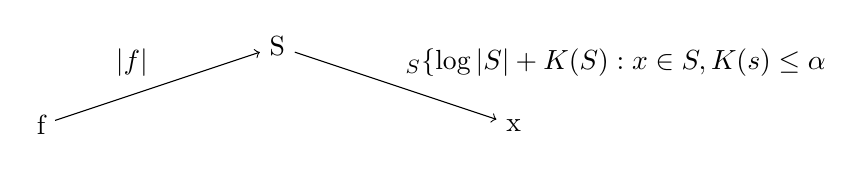
\begin{tikzpicture}[node distance=cm, auto]
  %\tikzstyle{every state}=[fill=red,draw=none,text=white]
  \node (f)  at (1,3)                  {f};
  \node (S)  at (4,4)                  {S};
  \node (x)  at (7,3)                  {x};
\path[->]  (f) edge  node   {$\argmin |f|$} (S);
\path[->]  (S) edge  node   {$\argmin_{S} \{\log|S| + K(S): x \in S, K(s) \leq \alpha$} (x);

\end{tikzpicture}

\caption{}
\end{figure}


Заметим, что решение задачи выбора модели в приведенном выше виде является вычислимой, то есть можно предложить алгоритм, вычисляющий данную задачу. Приведем схему данного алгоритма:
\begin{algorithmic}
\STATE Положим $\hat{p}, \hat{S}$ неопределенными;
\FORALL{$S, p: T(p) = S, |p| \leq \alpha$}
\IF{$\hat{S}$ неопределен или $|p| + \log(S) \leq \hat{p} + \log{\hat{S}},$}
\STATE  $\hat{p}, \hat{S} = p, S$
\ENDIF
\ENDFOR
\RETURN $\hat{S}$

\end{algorithmic}

Т.к. множество всех программ с длиной менее $\alpha$ является конечным, то алгоритм остановится, а потому вычислим. По построению он также доставлячет решение оптимизационной задачи~\eqref{eq:optim_ks_alpha}.

\begin{theorembd}
Обзначим за $S^{*}, K(S^{*}) \leq \alpha$  множество, доставляющее минимум следующей функции:
\[
    \delta(S) = \log{|S|} - K(x|S).
\]
Тогда  $\delta(S^{*}) - \delta{\hat{S}} = O(\log |x|).$
\end{theorembd}

Таким образом, пара $(\hat{p}, \hat{S})$ доставляет минимуму суммы $|p| + \log(S)$ при ограничениях на длину программы $|p| \leq \alpha$. Первое слагаемое данной суммы --- это длина  программы, то есть сложность описания множества $\hat{S}$. Сама сумма $|p| + \log(S)$ характеризует длину кода, требуемого для двухэтапного описания строки $x$, где на первом этапе мы описываем множество $S$, а на втором этапе находим $x$ во множестве $S$.

Описанный метод получения кода для описания выборки $x$ соответствует \textit{Принципу минимальной длины описания} или MDL: для заданной выборки требуется найти минимальный код, который описывает выборку (возможно, с некоторой наперед заданной допустимой ошибкой).

\subsection{Вероятностная интерпретация минимальной длины описания}
Рассмотрим подробнее задачу кодирования выборки. Задачу можно рассматривать как проблему передачу информации от кодировщика декодировщику. Задана выборка $\mathbf{X}, x \in \mathbf{X}$. Кодировщик кодирует информацию о выборке $\mathbf{X}$ с помощью некоторого кода $\mathbf{f}$ и передает ее декодировщику. Декодировщик декодирует код $\mathbf{f}(\mathbf{X})$, полученный от кодировщика и восстанавливает исходную выборку $\mathbf{X}$ (возможно, с некоторой потерей информации, если это оговорено заранее).
Допустим, для кодирования информации о выборке доступно несколько методов кодирования, при этом для разных объектов выборки минимальный по количеству информации метод будет отличаться. Тогда кодировщик должен передать не только информацию о выборке, но и информацию о самом методе кодировния. Проблему выбора оптимального способа кодирования из нескольких можно рассмотреть при помощи вероятностной интерпретации минимальной длины описания.
\begin{theorembd}
Пусть задан конечное или счетное множество $Z$ с введенной на нем вероятностью $P$. Тогда существует код $C$, такой что для любого $x \in Z$ длина его описания $L$ будет равняться  $L(C(x)) = -\log P(x)$.
\end{theorembd}

Таким образом, вместо методов кодирования можно рассматривать задачу выбора функции вероятности (правдоподобия?), введенной на признаковом описании выборки. Задача формулируется следующим образом:
\[
    \log p(\mathbf{X}|\mathbf{f}) + L(\mathbf{f}), 
\]
где $L(\mathbf{f})$ --- длина описания вероятностной модели $\mathbf{f}$. 


Одним из критериев качества вероятностного кодирования с помощью смеси кодов относительно фиксированного кодирования является регрет (TODO):
\[
R(x) =  - \log P(x) + \min_{\mathbf{f}} (\log P(x|\mathbf{f})).
\]
Регрет характеризует разницу между длиной рассматриваемого $\log P(x)$ кода для $x$ в сравнении с наилучшим кодом из некоторого множества $\mathbf{f}$.

Пусть модель $\mathbf{f}$ зависит от вектора параметра $\mathbf{w}$:
\[
    \log p(x|\mathbf{f}) = \log p(x|\mathbf{w}(x)),
\]
где $\mathbf{w}(x)$ --- оптимальные параметры для объекта $x$.

Тогда регрет выглядит следующим образом:
\[
R(P, x) =  - \log P(x) + \min_{\mathbf{w}} (\log P(x|\mathbf{w}(x)).
\]

Для всей выборки регрет определяется следующим образом:
\[
R(\mathbf{X}) =  \max_{x \in \mathbf{X}} (- \log P(x) + \min_{\mathbf{w}} (\log P(x|\mathbf{w}(w))).
\]


\begin{theorem}[(Штарьков, 1987)~\ref{mdl},\ref{shtarkov}]
Пусть велична
\[
    \log \sum_{x} p(x|\mathbf{w}(x))
\]
конечна.  Тогда следующее выражение доставляет единственный минимум регрета $R(\mathbf{X})$:
\[
    \frac{p(x|\mathbf{w}(x))}{\sum_{x' \in \mathbf{X}}p(x'|\mathbf{w}(x')) }.
\]
\end{theorem}
\begin{proof}
Рассмотрим выражение регрета для данной вероятностной меры:
\[
    - \log P(x) + \min_{\mathbf{w}} (\log P(x|\mathbf{w}(w)))  = \log \sum_{x} p(x|\mathbf{w}(x)).
\]
Выражение регрета не зависит от объекта выборки $x$. 
Заметим, что для любых двух отличных распределений  $p_1$, $p_2$ существует хотя бы один элемент, такой что 
\[
    p_1(x) < p_2(x).
\]
Действительно, пусть это неверно: $\forall x p_1(x) \geq p_2(x), \exists x': p_1(x) > p_2(x)$. Просуммируем вероятности $p_1$ и $p_2$ и воспользуемся тем, что сумма вероятностей по всем объектам будет равна единице:
\[
   1 =  \sum p_1  > \sum p_2 = 1,
\]
приходим к противоречию.

Тогда для любого распределения на выборке существует элемент $x'$:
\[
    \frac{p(x'|\mathbf{w}(x'))}{\sum_{x}p(\mathbf{w}|w(x)) } > p(x').
\]
Тогда 
\[
R(P, x)  \geq -\log p(x') + \log p(x'|\mathbf{w}(x')) > \frac{p(x'|\mathbf{w}(x'))}{\sum_{x}p(x|\mathbf{w}(x)) } = R(x).
\]

\end{proof}

Альтернативным методом выбора модели является двусвязный байесовский вывод.
На \textit{первом уровне} байесовского вывода находится апостериорное распределение параметров:
\begin{equation}
\label{eq:bayes}
    \hat{\mathbf{w}} = \argmax \frac{p(\mathbf{X}|\mathbf{w}, \mathbf{f})p(\mathbf{w}|\mathbf{f})}{p(\mathbf{X}| \mathbf{f}}),
\end{equation}
где $p(\mathbf{X}|\mathbf{w}, \mathbf{f})$ --- правдоподобие выборки при условии модели $\mathbf{f}$ с параметрами $\mathbf{w}$, $p(\mathbf{w}|\mathbf{f})$ --- априорное распределение параметров при условии модели $\mathbf{f}$. Оно задается на основе наших предположений о природе выборки и о способах ее порождения. Знаменатель $p(\mathbf{w}|\mathbf{f})p(\mathbf{X}| \mathbf{f})$ называется \textit{evidence} или \textit{обоснованность модели} и определяет, насколько хорошо модель способна описать выборку в среднем по всем возможным значениям параметров.


На \textit{втором уровне} байесовского вывода осуществляется выбор модели на основе обоснованности модели:
\[
\mathbf{f} = \argmax p(\mathbf{w}|\mathbf{f})p(\mathbf{X}| \mathbf{f}) = \int_{\mathbf{w}} p(\mathbf{X}|\mathbf{w}, \mathbf{f})p(\mathbf{w}|\mathbf{f}) d\mathbf{w}
\]
Эта величина также выступает байесовской интерпертацией минимальной длины. Для подтверждения этого факта докажем следующую теорему.

\begin{theorem}
Пусть правдоподобие $p(\mathbf{X}|\mathbf{w}, \mathbf{f})$ соответствует экспоненциальному семейству распределений, т.е.
\[
    p(x|\mathbf{w}, \mathbf{f}) = h(x)g(\boldsymbol{\eta}) \text{exp}\left(\boldsymbol{\eta} \cdot \mathbf{T}(x)\right),
\]
где $h, g, \mathbf{T}$ --- некоторые функции, $\boldsymbol{\eta}$ --- некоторый параметр распределения.

Пусть в качестве априорного распределения выступает распределение Джефри:
\[
    p(\mathbf{w}|\mathbf{f}) = \frac{\sqrt{I}}{\int_w \sqrt{I(w)}}, \text{ где } I  \text{---определить матрицы Фишера:}    
\]
\[
    I(\mathbf{w}) = \text{det}\{\mathsf{E}_w \frac{-\partial^2}{\partial w_i \partial w_j } \log p(\mathbf{X}|\mathbf{w}, \mathbf{f}) \}_{ij}.
\]
Тогда регрет можно аппроксимировать следующим выражением:
\[
\frac{k}{2}\log{\frac{n}{2\pi}} - \log p(\mathbf{X}|\mathbf{w}, \mathbf{f}) + \log \sqrt{I(\mathbf{w})}.
\]

\end{theorem}

\begin{proof}
Воспользуемся аппроксимацией Лапласа для упрощения формулы обоснованности модели.
Разложим $\log p(\mathbf{X}, \mathbf{w}|\mathbf{f}) = \log p(\mathbf{X}|\mathbf{w},\mathbf{f})p(\mathbf{w}|\mathbf{f})$ в точке локального максимума $\mathbf{w}_0$ в ряд Тейлора:
\[
    \log p(\mathbf{X}, \mathbf{w}|\mathbf{f}) \approx \log p(\mathbf{X}, \mathbf{w}_0|\mathbf{f})  - \frac{1}{2} (\mathbf{w}-\mathbf{w}_0)^\T \mathbf{A} (\mathbf{w}-\mathbf{w}_0),
\]
\[
    A_{ij} = -\frac{\partial^2}{\partial w_i \partial w_j}\log p(\mathbf{X}, \mathbf{w}|\mathbf{f})|_{\mathbf{w} = \mathbf{w}_0}.
\]

Полученное распределение представимо в виде ненормированного гауссового распределения. для такой аппроксимации плотности вероятности запишем нормирующий коэффициент: 
\[
    \log p(\mathbf{X}, \mathbf{w}|\mathbf{f}) \approx \log p(\mathbf{X}|\mathbf{w}_0, \mathbf{f}) + p(\mathbf{w}_0|\mathbf{f}) - \log \sqrt{\frac{(2\pi)^k} - {\det \mathbf{A}}}.
\]

Подставляя в полученную формулу распределение Джеффри получим:
\[
    p(\mathbf{X}, \mathbf{w}|\mathbf{f}) \approx p(\mathbf{X}|\mathbf{w}_0, \mathbf{f}) - \log\sqrt{\frac{(2\pi)^k}{2}}.
\]
TODO: там еще информация Фишера + экспоненциальное семейство.
Тогда регрет будет равен:
\[
    R(P, x) \approx  \log\sqrt{\frac{(2\pi)^k}{2}}.
\]
\end{proof}

\begin{theorembd}
При количество параметров, стремящемся к бесконечности, регрет оптимальной модели отличается от байесовской оценки на константу:
\[
R(P, x) = \frac{k}{2} \log \frac{n}{2\pi} + \log{\int_{\mathbf{w}}} \sqrt{I(\mathbf{w}} d\mathbf{w} + o(1).
\]
\end{theorembd}

TODO: вывод, что эти вещи совпадают.
\begin{thebibliography}{99}
\bibitem{kolmogorov}
	Успенский В., Шень А., Верещагин Н. Колмогоровская сложность и алгоритмическая случайность. – Litres, 2017

\bibitem{grun_ks}
Grunwald P., Vitányi P. Shannon information and Kolmogorov complexity //arXiv preprint cs/0410002. – 2004.

\bibitem{ks_struct}
Vereshchagin N. K., Vitányi P. M. B. Kolmogorov's structure functions and model selection //IEEE Transactions on Information Theory. – 2004. – Т. 50. – №. 12. – С. 3265-3290.

\bibitem{mdl}
Grunwald P. A tutorial introduction to the minimum description length principle //arXiv preprint math/0406077. – 2004.

\bibitem{shtarkov}
Штарьков Ю. М. Универсальное последовательное кодирование отдельных сообщений //Проблемы передачи информации. – 1987. – Т. 23. – №. 3. – С. 3-17.
\end{thebibliography}

\end{document}

